\chapter{Implementation}
\label{Chapter4}
\lhead{Chapter 4. \emph{Implementation}} % Write in your own chapter title to set the page header

In order to test our proposed energy-aware gossip broadcasting protocol, we developed this protocol in open-source software Network Simulator 3 (ns-3). 

To achieve the goals stated in section~\ref{sec:problem}, I took four crucial steps.

We applied Depth First Search (DFS) algorithm to ensure that all nodes in the network are connected in some way. Thus we eliminated the possibility that a network is separated into two subnets such as shown in Figure~\ref{fig:twoSepNet}. 

\begin{figure}
	\centering
	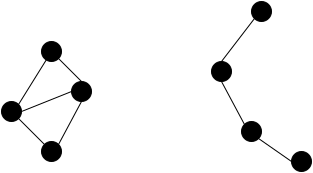
\includegraphics[width=3in]{twoSepNet.png}
	\caption{An example when two separate subnets formed}
	\label{fig:twoSepNet}
\end{figure}


\begin{itemize}
	\item Extend the Internet Control Message Protocol (ICMP) to support transmitting three simple control messages needed for gossip protocol.
	\item Develop the gossip protocol application to be installed on network nodes.
	\item Set wireless ad-hoc network attributes and gossip protocol attributes, which has already be presented in section~\ref{sec:problem}.
	\item Import nodes connectivity information from topology files and export simulation results for performance evaluation.
\end{itemize}

\subsection{ICMP Extension}

ICMP stands for Internet Control Message Protocol. The most common use of ICMP is for error reporting~\cite{james}. A ICMP message contains two parts: 8-byte header and data section. The first 4 bytes of the header have fixed format. However, the last 4 bytes vary and depend on the type or code of the ICMP packet~\cite{forouzan}. The first and second byte of the header is the type field and code field respectively. And the third and fourth byte are checksum field. The format of the header is shown in table \ref{table:1}.

\begin{table}[h!]
	\centering
	\caption{ICMP Header Structure}
	\label{table:1}
	\begin{tabular}{|p{1 cm}|p{1 cm}|p{1 cm}|p{1 cm}|p{1 cm}|}
		\hline
		Octet & 0 & 1 & 2 & 3 \\
		\hline
		& Type & Code & 
		\multicolumn{2}{ |c| }{Checksum}  \\
		\hline
		Octet & 4 & 5 & 6 & 7 \\
		\hline
		& 
		\multicolumn{4}{|c|}{Rest of Header}  \\
		\hline
	\end{tabular}
\end{table} 

Table \ref{table:2} here presented some selected ICMP message types. 

\begin{table}[h]
	\centering
	\caption{Control Messages}
	\label{table:2}
	\begin{tabular}{|p{1.5cm}|p{0.8 cm}|p{4.5 cm}|}
		\hline
		Type & Code & Description \\                                                           
		\hline
		0  & 0   & Echo reply   \\ \hline
		8  &  0 & Echo request \\ 
		\hline
		9 & 0 & Router Advertisement \\
		\hline
		10	& 0	&	Router discovery/selection/solicitation \\
		\hline
		42 to 255    &   & Reserved    \\ 
		\hline
	\end{tabular}
\end{table}

Since type 42 to 255 are reserved for further development, I decided to extend ICMP by defining type 42, 43, and 44 to represent acknowledgment packet, request packet, and data packet respectively. The detail is shown in table \ref{table:3}.

\begin{table}[h]
	\centering
	\caption{Gossip Protocol Control Messages}
	\label{table:3}
	\begin{tabular}{|p{0.8cm}|p{0.5 cm}|p{3.5 cm}|}
		\hline
		Type & Code & Description \\                                                           
		\hline
		42  & 0   & Send Acknowledgment   \\ \hline
		43  &  0 & Send Request \\ 
		\hline
		44 & 0 & Send Data \\
		\hline
	\end{tabular}
\end{table}

Upon these new control message types extension, we could further develop gossip protocol in NS-3.



Topology wise, nodes are randomly place in a square area which is proportional to the number of nodes. The equation to calculate the size of the square is as follows:

(Insert the equation here).

Every node's coordinates are used to calculate neighbors list for each node. In practice, the global access of this information is usually not easy to obtain. Thus, Hello packets are used to compile neighbors list for each node.

Because nodes are randomly placed in a square area, with fixed WiFi range there could be a case that each node has at least one neighbor but the network is separated into two subnets unconnected. [twoSepNet.png]

Therefore, I used an algorithm that uses depth-first search algorithm to determine whether all nodes get visited during the recursive search. If the algorithm successfully traverse all nodes, it is considered a complete graph which means the network is connected. If the algorithm yield a failure, this trial will be rejected and the simulation will move on to next trial.

In order to collect benchmark of adaptive fanout gossip protocol, one extra node is place in the area. Its functions are generate new packets, collect other nodes' received time of every packets, and store new packets generate time. A trimmed version of adaptive fanout gossip protocol is used to generate new packets. An UDP server application is installed on the node to collect other nodes' received time of every packets.

Adaptive fanout gossip protocol is installed on all other nodes in the network. Besides that, a UDP client application is also installed on them to send received time of every packet. The simulation stops when any one node's energy is depleted. After that, all the data collected is processed to generate our performance metrics. 

\section{Performance Metrics}
Life Span of the Network

Definition: The time when any node's battery die

Because the goal of this protocol is to broadcast any new packet, the network will lose the physical ability whenever any node lost wireless connection to its neighbors due to energy depletion. Therefore, this metric indicates how long a network with size n could stay connected using a broadcast protocol.

Average Packet Broadcast Time

Let's think about broadcasting one packet from one node to (n-1) nodes, the packet broadcast time of this packet for this network is the difference between the time when last node received the packet and the time this packet was first sent.

Because for each independent trial, multiple packets will be sent. The packet broadcast time is calculated for each packet in the way described above. In the end, we average the times for each scenario (e.g. n = 10). 

Need to develop a mathematical equation for this

The average packet broadcast time indicates the time needed for a packet to reach every node in the network.

Protocol Overhead

There are three types of protocol packets for the protocol. The ack packet, solicit packet, and the payload packet. The acknowledgment packet is sent to the sender from receiver when a node received a payload that it already received before. The solicit packet is sent to query a random neighbor for its latest payload. For example, in one trial with n nodes, if it broadcaster m packets, then the average protocol overhead is defined as:

$overhead = ()(p1 + p2 + … + p_n) / n) / m$

This metric indicated how many packets is needed for a node to facilitate broadcasting one packet. 

Consumed Energy

The consumed energy per node per packet is defined as

energy = ((e1 + e2 + … + en)/n)/m

This metric measures the amount of energy needed for a node to facilitate broadcasting one packet. 


\subsection{Gathering Simulation Data}

To evaluate the performance of gossip protocol, we use several randomly generated topology files with the number of nodes as variable. Those topology files are derived from a random geometric graph network, which was created by uniformly and randomly placing nodes into a space and then connect nodes whose distance is smaller than some given radius.

\begin{figure}
	\centering
	\begin{verbatim}[fontsize=\small]
	#Nodes
	0
	1
	2
	#Edges
	(0, 1)
	(1, 2)
	\end{verbatim}
	\caption{A topology file of a linear topology with three nodes.}
	\label{fig:topsimple}
\end{figure}


Each topology file contains the number of nodes as well as all the edges, which represents the connections between nodes. As an example, the content of a simple topology file is shown in figure~\ref{fig:topsimple}. A parser written in C++ is developed to create the given number of nodes in NS-3 and installed the gossip protocol application on them. Thereafter, all edges are parsed and created accordingly. Each node holds an NS-3 Ipv4Interface with assigned Ipv4 address and stores the Ipv4 addresses of his neighbors.

For the simulation, we set the link rate for all connections to be 1Mbp. Also, all nodes are instructed to execute the gossip process of sending out data periodically every 5ms. The interval of requesting new data is set to 5s.

To allow the performance analysis, all nodes count the number of data packets they sent. All nodes would track how many hops the data message experienced before reaching them and they record the time when they received the data message as well. For every single simulation, we collect the information from the nodes and determine the average amount of data packets sent per node and average number of hops per node. Moreover, the information about how long it took for the message to reach the ``last'' node is also recorded.

This information is determined and stored for each of the several hundred topology files. It should be noted that due to time limitations each topology file was only simulated once. Finally, we did statistical analysis upon those collected data in the hope of verifying the assumptions we made in section~\ref{sec:problem}.

